\section{Sensorik}
Da wie oben beschrieben die Sensorik ein große Rolle im Bereich der IoT spielt, sind in diesem Kapitel die Grundlagen der Sensorik aufgeführt.  
\subsection{Allgemein}
Der Begriff \textit{Sensorik} kommt aus dem Latein. \textit{Sensus} bedeutet "der Sinn". Generell lässt sich sagen, dass ein Sensor ein System ist, dass eine physikalische Größe und deren Änderung misst und die Messung in nutzbare Signale wandelt. 
Regelungen können Sensoren als Messerichtungen nutzen.  

\begin{figure}
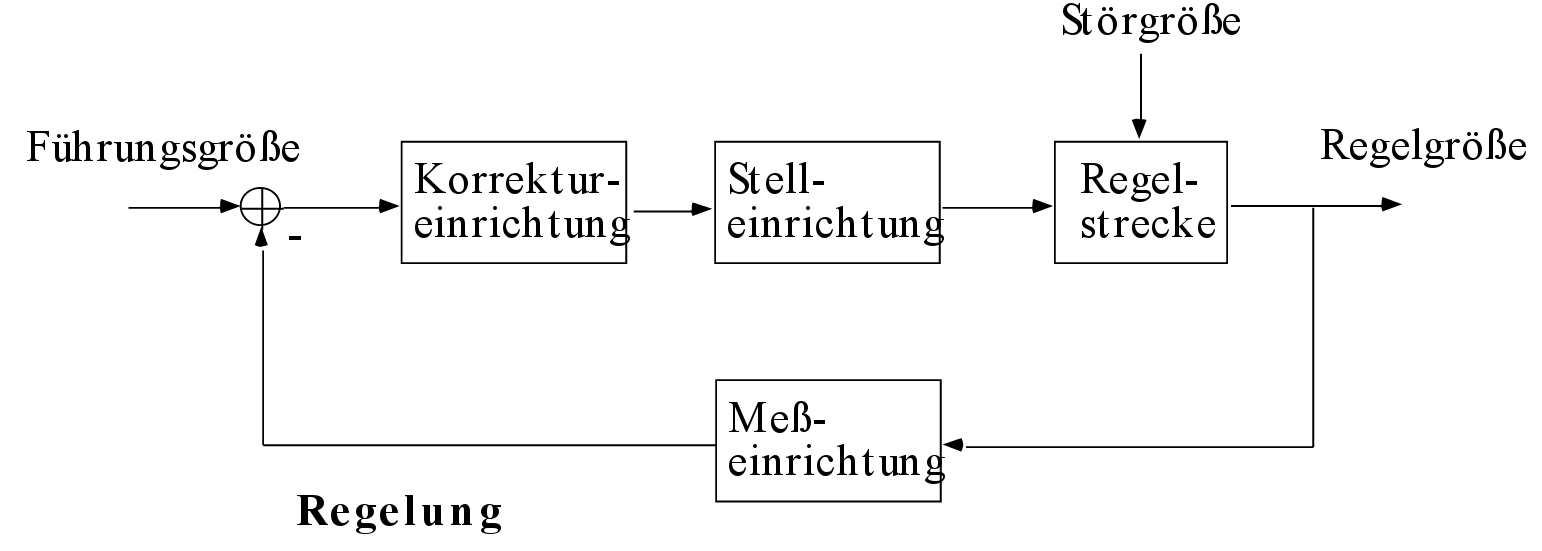
\includegraphics[scale=0.3
]{bilder/regelung} 
\caption{Schema einer Regelung Quelle: TODO Strand}
\label{IPv4}
\end{figure}

Sensoren kann man in folgende Kategorien einteilen:
\begin{itemize}
\item Mechanische Sensoren
\item Temperatursensoren 
\item Chemische Sensoren
\item Biosensoren
\item Optische Sensoren 
\item Akustische Sensoren
\item Magnetische Sensoren 
\item Gassensoren
\end{itemize}

Mechanische Sensoren können beispielsweise Kontaktsensoren sein. Sie können zum benutzt werden um zu erkennen, ob eine Tür geschlossen ist. Chemische Sensoren können chemische Stoffe quantifizieren. Der Unterschied zu Biosensoren ist, dass diese meist organische Verbindungen messen können (zum Beispiel Glucose). 

Sensoren können unterschiedlich Komplex sein, je nach Anwendungsgebiet. Man unterscheidet zwischen:
\begin{itemize}
\item Elementarsensoren
\item Integrierten Sensoren
\item und Intelligenten Sensoren.
\end{itemize}

Elementare Sensoren sind man einfachsten aufgebaut. Im Falle eines optischen Sensors kann dieser aus leidlich einer Photozelle bestehen. Das Signal das er zurück gibt, muss unter Umständen ein A/D-Wandler noch digitalisieren. 
Ein Integrierter Sensor ist da schon komplexer. Er bereitet sein Signal auf. Das kann beispielsweise eine Verstärkung oder eine Filterung sein. Bei einem Intelligenten Sensor redet man schon von einem Rechner. Es kann sich zum Beispiel um eine Kamera oder um einen Laserscanner handeln. Derartige Sensoren arbeiten mit einer umfassenden Vorverarbeitung der Daten. 
Ferner unterscheidet man zwischen internen und externen Sensoren. Im weiteren betrachten wir die externen Sensoren. Sie sind in der IoT-Welt von hoher Bedeutung.
%TODO Quelle Strand
\subsubsection{Temperatursensoren}
\begin{figure}
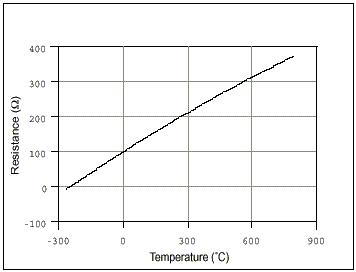
\includegraphics[scale=1]{bilder/pt100} 
\caption{PT100 Temperatursensor Quelle TODO https://www.mikrocontroller.net/articles/Temperatursensor }
\label{PT100}
\end{figure}
Die Temperatur lässt sich auf viel Art und Weisen berechnen. Sensoren für Mikrocontroller kann man in zwei Kategorien einteilen:
\begin{itemize}
\item Analoge Sensoren
\item Digitale Sensoren
\end{itemize}
Ein gängiger analoger Temperatursensor ist der \textit{PT100}. Es handelt sich hierbei um einen Platinwiderstand. Er hat bei null Grad Celsius einen Widerstand von 100 Ohm. Der Widerstand nimmt ungefähr 0,4 Ohm pro einem Grad Temperaturänderung zu. Ein Vorteil dieses Sensors ist es, dass er einen großen Messbereich hat. Generell benötigt man für derartige Temperatursensoren eine relativ komplexe Schaltung. Außerdem kann kann man mit dem Sensor einen relativ großen Temperaturbereich abdecken.

https://www.mikrocontroller.net/articles/Temperatursensor
\section{Luftfeuchtigkeit}



Temperatur
Luftfeuchtigkeit
Beleuchtungsstärke
Luftdruck
Bewegungsmelder
Bodenfeuchtete

 
